\documentclass[conference]{IEEEtran}
\usepackage{times}

% numbers option provides compact numerical references in the text. 
\usepackage[numbers]{natbib}
\usepackage{multicol}
\usepackage[bookmarks=true]{hyperref}

\usepackage[pdftex]{graphicx}
\usepackage{comment}

\usepackage{algorithm}
\usepackage[noend]{algpseudocode}

\usepackage{amsfonts}
\usepackage{amsmath}

\usepackage{amsthm}
\newtheorem{thm}{Theorem}
\newtheorem{lem}{Lemma}
\newtheorem{asmp}{Assumption}
\newtheorem{defn}{Definition}

\pdfinfo{
   /Author (Homer Simpson)
   /Title  (Robots: Our new overlords)
   /CreationDate (D:20101201120000)
   /Subject (Robots)
   /Keywords (Robots;Overlords)
}

\begin{document}

% paper title
\title{ MORRF$^{*}$ : Sampling-Based Multi-Objective Motion Planning }

% You will get a Paper-ID when submitting a pdf file to the conference system
\author{Author Names Omitted for Anonymous Review. Paper-ID [add your ID here]}

\maketitle

\begin{abstract}
The importance of multi-objective path planning emerges with the increase of the requirement complexity of the tasks assigned to the robot.
The nature of the path planning problem makes that a few of the multi-objective optimization methods could not be directly imported to find the Pareto optimal solutions.
Inspired by the RRT* and the decomposition-based multi-objective optimization, we proposed a MORRF*(Multi-objective Rapidly exploring Random Forest*) in this paper that could effectively and efficiently find the Pareto optimal set of solutions.
The RRF consists of two types of tree structures, the reference tree and the subproblem tree.
Each reference tree explores a single objective to support the estimation of an Utopia position in the fitness space.
Each subproblem tree explores to find a solution to the assigned subproblem.
The solutions from all the trees form a set of Pareto optimal solutions. 

Theoretical analysis has been shown to support the feasibility of this algorithm and the asymptotic optimality. 
Simulations have been take to show the effectiveness and the efficiency of the MORRF*.
\end{abstract}

\IEEEpeerreviewmaketitle

\begin{comment}
Final Paper Submission Deadline: January 22, 2015, 23:59 PST

Papers can be up to 8 pages + references. 
This means that if more than 8 pages are used, the 9th and subsequent pages should contain ONLY references. 
The length requirement will be strictly enforced.
\end{comment}

\begin{comment}


\end{comment}

\section{Introduction}
\label{sec:intro}

\begin{comment}
(1) Why the multi-objective path planning is needed 
(2) Why the multi-objective path planning is hard (compare with a common multi-objective optimization problem)
\end{comment}

In many real applications of the robots, the complexity of tasks inherently implies more than single objective to be reached.
A robot in a search task is usually expected to maximize the search coverage with a consideration of the energy efficiency so that the execution time could also be expanded~\cite{yi2014supporting}. 
If there exists risk in the working environment, the robot should also try to avoid dangerous regions.
In robot arm manipulation planning, there usually exist several criteria to be considered as well~\cite{Pires2004}, for example, movement, joint velocities, joint accelerations and etc. 
The most commonly applied method is converting into a single objective by linearly weighted summation of multiple objectives.
The performance of the planned paths relies strongly on how different objectives are weighted.
The difficulty becomes how the task supervisor should assign the weights.
Meanwhile, the multiple objectives in a planning optimization are sometimes incomparable or unrankable.
It becomes impossible to assign weights or ranks.
Finding a set of non-dominant solutions is introduced to answer the multi-objective optimization.
A non-dominant solution means that there exists no other solution can surpass it in all the objectives.
A human interactive process can help the decision maker finding the most preferred solution, especially when the decision maker's preference is hard to precisely describe.
This has been applied well in optimal design and optimal decision already.

However, how to find Pareto optimal paths in the multi-objective path planning has not been well answered yet.
The popular methods in multi-objective optimization are hard to be directly applied to path planning problems.
One way is coding a path into a fixed-length set of segments, which can be represented by direction~\cite{Ahmed2013} or way points~\cite{5160222}~\cite{Pires2004}.
Evolutionary algorithms could then be imported to search the optimal solutions.
In order to have a better approximation, the number of the segments consisted of a path cannot be too small.
This will make the solution search working in a rather high dimension solution space.
Even some algorithms work efficiently in high dimension solution spaces, 
forcing different path trajectories represented by fixed number of segments is hard. 
Because naturally the total length and the details of curvatures can be versatile.
Many constraints of the problems are then difficult to be modeled.
It is hard to estimate how many segments would be enough to represent all the possible paths due to difference in shapes and the sizes of the obstacles.
Allowing different segment numbers of the paths could help but the solution format won't fit the requirement of most of the evolutionary algorithms.
Also, when modeling a path into a point in a solution space, the obstacles in the working space could make a few of infeasible regions, which influences the continuity and increases the hardness of the heuristic-based search~\cite{5160222}~\cite{4358754}.

While the path planning on continuous space is of a over big search space, 
RRT(Rapidly exploring Random Tree) is a popular algorithm in finding feasible solutions from a start position to a goal position, which supports well in the environments with complex obstacles. 
The tree structure also guarantees a great efficiency on path search.
RRT* was recently introduced and has been proven to effectively finding an optimal path given enough sampling time~\cite{Karaman:2011:SAO:2000201.2000209}~\cite{Karaman.Frazzoli:RSS10}.
Similar with that decomposing the multi-objective optimization problem into a few subproblems in \cite{4358754}, we propose the MORRF*(Multi-Objective Rapidly exploring Random Forest*) to find a set of Pareto optimal paths from the start position to the goal position.

In this paper, we reviews a few existing multi-objective path planning algorithms and the works that inspires our algorithm in Section \ref{sec:related_works}.
With the definition of the multi-objective path planning problem, MORRF* is introduced and explained in Section \ref{sec:morrt}.
We provide theoretic analysis to support MORRF* in Section \ref{sec:theoretic_analysis}.
Simulation results are given in Section \ref{sec:simulation} to illustrate the performance of the proposed algorithm.

\section{Related works}
\label{sec:related_works}

Finding a set of Pareto optimal paths replies on exploring the non-dominance of the paths.
The implicit comparative property prevents a few pruning techniques for efficiency and the problem complexity would be greatly extended as a result.
Discretizing the space is one way to reduce the problem complexity.
By modeling the working space into the connectivity of a graph structure, a multi-objective A* search could be applied to find the solution set in \cite{Mandow:2005:NAM:1642293.1642328}.
Another approach is coding the path into a sequence of directions from one cell to next cell after map discretization.
NSGA-II can then be used to find a set of Pareto optimal solutions in \cite{Ahmed2013}.
The solutions would be translated into sequences of way points.
Planning on a discretized map is never the best way of finding the optimal path.
Either a coarse discretization loses the detail information, or a fine discretization brings too much redundancy and complexity.
Especially when there exists obstacles in the working space, a sequence of way points might not be enough to represent a path.
A direct line connecting two points might get into obstacles and is not feasible.  
Therefore, spline are introduced to interpolate a sequence of way points into a trajectory in \cite{6181426}.
How the interpolated shapes is actually not evaluated in the optimization process. 
The solutions are not directly answer to the defined path planning problems.
Increasing the path resolution, the number of the steps, should better deal with the obstacles in the working space and also follows better along the gradient of the fitness.
But the dimension of the solution space would be increased.
It also reveals that approaching the problem in a continuous space would be better.

The biggest challenge to multi-objective evolutionary algorithms on high dimension continuous space is efficiency.
Within a small search step means that it will take much longer time to converge to the Pareto front.
But within a big search step is likely to miss the optimal solutions.
As a path is denoted by a point in a high dimension continuous space, the exist of obstacles that makes plenty of paths infeasible leads to plenty of undefined regions in the continuous space.
This leads to the discontinuity of the solution space, which could impact the performance of many evolutionary algorithm on multi-objective optimization.

Sampling-based path planning works effectively in continuous space.
RRT(Rapidly exploring random tree) has been one of the most popular tools, which  efficiently explores the space by randomly sampling and works well with any complex obstacles.
The simplicity of the algorithm shortens the search time of a feasible solution.
However, in finding an optimal solution, it is figured that RRT will fail in \cite{Karaman.Frazzoli:RSS10}.
Thus RRT$^{*}$ is introduced to facilitate the optimal search.
A \emph{Rewire} process is imported to update the tree structure gradually towards optimality which is triggered by new samplings.
The asymptotic optimality of RRT$^{*}$ has been proven in~\cite{Karaman.Frazzoli:RSS10}~\cite{Karaman:2011:SAO:2000201.2000209}.
The structure is update with new samplings, and the connections are updated with the cost update.
Gradually it learns the optimal path from each vertex of the tree structure to the start position.
Figure \ref{fig:RRTstar2} gives an example.
\begin{figure}
\centering
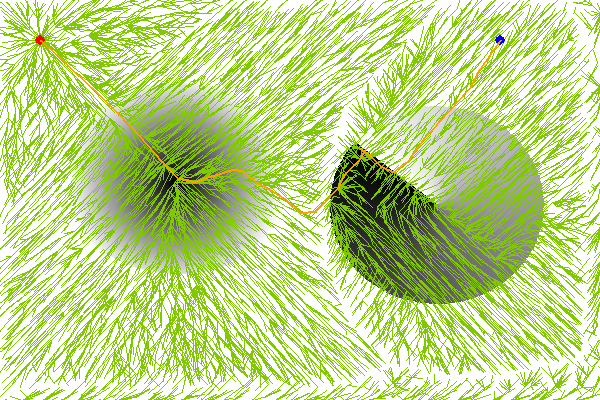
\includegraphics[width=0.9\linewidth]{fig/RRTstar2}
\caption{Tree structure after exploring fitness space.}
\label{fig:RRTstar2}
\end{figure}

In find Pareto optimality, decomposition method is another effective way besides dominance comparison.
MOEA-D is proposed in \cite{4358754}, which decomposes a multi-objective optimization problem into a class of subproblems.
Let $ \vec{\lambda} = [ \lambda_{1} , \cdots , \lambda_{K}  ]^{T} $ be a weight vector and $ \sum_{k=1}^{K} \lambda_{k} = 1 $.
Three types of decomposition methods are introduced in \cite{4358754}.
\begin{itemize}
\item \emph{Weighted sum approach} \\
Maximize $ g^{ws} (x \mid \vec{\lambda}) = \sum_{k=1}^{K} \lambda_{k} f_{k} (x) $;
\item \emph{Tchebycheff approach} \\
Minimize $ g^{te} (x \mid \lambda , z^{*}) = \max_{i \leq k \leq K}  \{ \lambda_{i} | f_{k}(x) - z^{*}_{k}  | \} $;
\item \emph{Boundary intersection approach} \\
Minimize $ g^{bi} (x \mid \lambda , \vec{z}^{*} ) = d $, subject to $ \vec{z}^{*} - F(x) = d \lambda $.
\end{itemize}
The solutions of all the subproblems are a subset of the Pareto optimal set.
A few evolutionary algorithms based on the decomposition method are proposed to solve the multi-objective optimization~\cite{6600851}, 
especially in many-objective optimization problems.
It is noticeable that the decomposition depends on finding the ``Utopia'' reference vector $ \vec{z}^{*} = [z^{*}_{1}, \cdots , z^{*}_{K}]^{T} $ as a reference to minimize different weighted distances.
In the next section, we will propose an algorithm that explores the solution spaces parallel using RRT* tree structure.
Instead of a single tree structure, a set of trees are constructed in the exploration process.
Thus it is named MORRF$^{*}$ (Multi-objective Rapidly exploring Randm Forest$^{*}$).



\section{Multi-Objective Rapidly exploring Random Forest$^{*}$}
\label{sec:morrt}

When the multi-objective path planning problem is defined on a continuous space $ X $, the Pareto optimal set is not enumerable.
The target becomes finding a finite subset of the Pareto optimal set.
The diversity of the solution is expected to be maximize so that the Pareto optimal set can be better approximated.
In this paper, we only look at the minimization problem, which means all the objectives are expected to be minimize.
Let the size of the finite subset be $ M $.
We could have the multi-objective path planning problem defined.
\begin{defn}{ \textbf{Multi-Objective Path Planning} }
Given a bounded connect open set $ X \subset \mathbb{R}^{d} $, an obstacle space $ X_{obs} $, an initial state $ x_{init} $, and a goal region $ X_{goal} $.
The obstacle-free space is $ X_{free} = X \setminus X_{obs} $.
Given $ K $ objectives that are determined by a vector function
$ \vec{F}(x) = [ f_{1} (x), \cdots , f_{K}(x) ]^{T} : \mathbb{R}^{d} \rightarrow \mathbb{R}^{K} $ and 
$ \vec{F}(\sigma) = \sum_{x \in \sigma} \vec{F}(x) $.
Find $ M $ paths $ \sigma^{*} \in \Sigma^{*}  : [0, s] \rightarrow cl(  X_{free} ) $ such that
\begin{itemize}
	\item $ \sigma^{*} (0) = x_{init} $ and $ \sigma^{*} (s) = X_{goal}  $;
	\item $ \not \exists \sigma , \forall k \in K, f_{k} (\sigma) > f_{k} (\sigma^{*}) $.
\end{itemize}
\end{defn}

Similar with MOEA-D~\cite{4358754}, the solution set of size $ M $ is obtained by decomposing the multi-objective problem into $ M $ subproblems.
Each subproblem is assigned with a tree structure to explore the solution space.
The solve of the subproblem relies on the knowledge of the reference vector $ \vec{z}^{*} $ in the fitness space if we follow the Tchebycheff approach or Boundary intersection approach.
In this paper, for simplicity, we only look at the Tchebycheff approach.
Boundary intersection approach could be easily implemented with slight modification.
Thus $ K $ trees are introduced to explore the minimum of each objective.

\begin{figure}
\centering
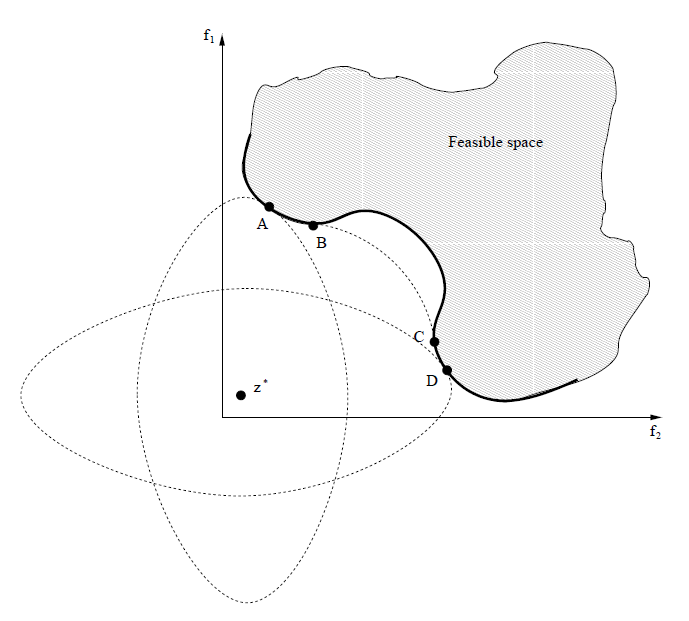
\includegraphics[width=0.9\linewidth]{fig/Tchebycheff}
\caption{Tchebycheff method of finding Pareto front.}
\label{fig:Tchebycheff}
\end{figure}

There are two types of tree structures used for the optimization process.
\begin{itemize}
\item Each \emph{reference tree} explores for a single objective $ f_{k} (x), k \in K $. 
The fitness of each vertex is calculated from the $ k $-th objective.
\item Each \emph{subproblem tree} explores for a subproblem $ g_{m} ( x \mid \lambda_{m} , z^{*} ) , m \in M $.
The fitness of each vertex 
\end{itemize}
In each iteration, a new position is generated from random sampling and the collision check.
The new position is firstly added to all the reference trees to update the structure and refine the costs of neighboring vertices.
Then the new position is added to all the subproblem trees to explore the subproblem in a similar way with RRT$^{*}$.
Like the RRT and RRT$^{*}$, when the algorithm stops, each subproblem tree returns a path.
The paths from all the subproblem trees forms the solution set.
The exploration at each iteration is given in Algorithm \ref{alg:rapidly_exploring_process}.

%Because the convergence of the tree structure in RRT* means that the path from the root to any vertex is an optimal path of the defined cost.
%We use the same sampling position to extend all the trees in one iteration.
%Thus the vertices in the reference trees could be used as reference for estimating the cost in constructing the subproblem trees.
In each iteration, sample new position is used to extend both all the reference trees and all the subproblem trees.
This enables us to estimate the fitness of each vertex in the subproblem tree by using the estimated reference vector of the vertex.
The reference vector of the vertex is obtained by vectorizing the fitness of corresponding vertices (same position) in $ K $ reference trees.
It means all the trees in MORRT$^{*}$ have same vertices but the edges are different.
The edge are determined by the definition of the fitness in each tree.

%Like all the sampling-based optimization, the random positions are uniformly sampled from the workspace.
%It means that all the tree have equivalent vertices constructed from same positions set sequentially.
%But they are connected by different measurements of the costs, either a single objective or a cost from subproblem definition.
%The edges of the trees can be different.

\begin{figure}[H]
\centering
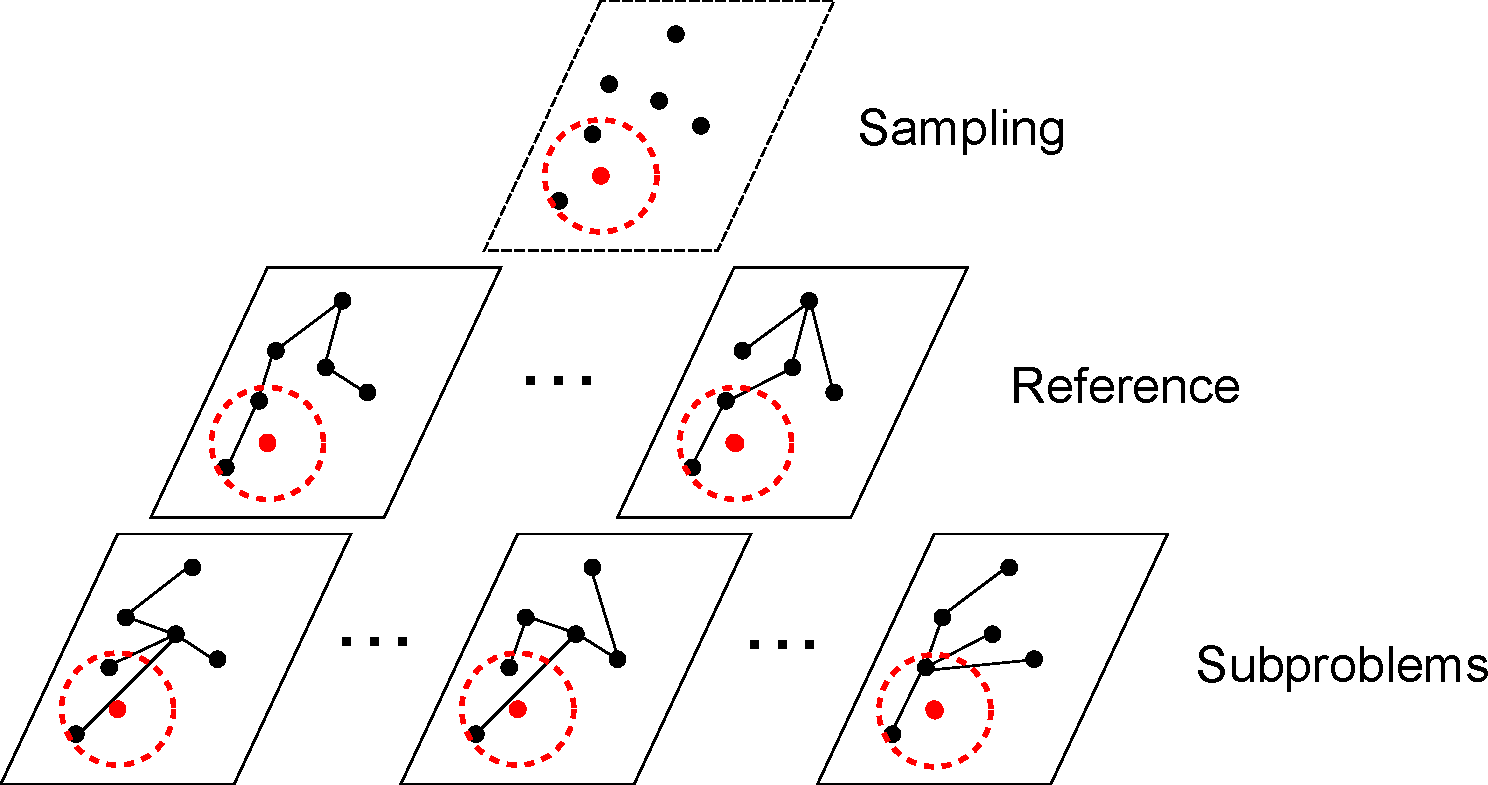
\includegraphics[width=0.9\linewidth]{./fig/MORRTstar}
\caption{Rapidly Exploring Process}
\label{fig:MORRTstar}
\end{figure}

\begin{algorithm}
	\label{alg:rapidly_exploring_process}
	\begin{algorithmic}[1]
		\For{ \textbf{each} $ V_{r} \in \mathbf{V}_{r} $ } 
		\State $ V_{r} \leftarrow \{ x_{init} \} $; $ E_{r} \leftarrow \emptyset $; $ i \leftarrow 0 $
		\EndFor
		\For{ \textbf{each} $ V_{s} \in \mathbf{V}_{s} $ } 
		\State $ V_{s} \leftarrow \{ x_{init} \} $; $ E_{s} \leftarrow \emptyset $; $ i \leftarrow 0 $
		\EndFor
		\While{ $ i < N $ }
		\For{ \textbf{each} $ G_{r} \in \mathbf{G}_{r} $ } 
		\State $ G_{r} \leftarrow (V_{r}, E_{r}) $
		\EndFor
		\For{ \textbf{each} $ G_{s} \in \mathbf{G}_{s} $ } 
		\State $ G_{s} \leftarrow (V_{s}, E_{s}) $
		\EndFor
		\State $ x_{rand} \leftarrow $ \Call{ Sample }{$ i $} ; $ i \leftarrow i + 1 $
		\State $ V' \leftarrow V $; $ E' \leftarrow E $
		\State $ x_{nearest} \leftarrow $ \Call{Nearest}{$ G, x $}
		\State $ x_{new} \leftarrow $ \Call{Steer}{$ x_{nearest}, x $}
		\If{ \Call{ObstacleFree}{$ x_{nearest}, x_{new} $} }
		\For{ \textbf{each} $ G_{r} \in \mathbf{G}_{r} $ } 
		\State $ (V_{r}, E_{r}) \leftarrow $ \Call{ Extend$_{Ref}$ }{$ G_{r}, x_{new} $}
		\EndFor
		\For{ \textbf{each} $ G_{s} \in \mathbf{G}_{s} $ } 
		\State $ (V_{s}, E_{s}) \leftarrow $ \Call{ Extend$_{Sub}$ }{$ G_{s}, x_{new} $}
		\EndFor
		\EndIf
		\EndWhile
	\end{algorithmic}
	\caption{Multi-objective Rapidly Random exploring }
\end{algorithm}

We have the definitions of several functions similar with the definitions in ~\cite{Karaman.Frazzoli:RSS10}.
\begin{itemize}
	\item \textbf{Sampling} - \textsc{Sample}() \\
	It returns independent identically distributed samples from $ X_{\mbox{free}} $.
	\item \textbf{Steering} - \textsc{Steer}() \\
	Given two points $ x $ and $ y $, it returns a point $ z $ that its distance to $ x $ is less than $ \eta $ and minimizes the distance to $ y $. 
	\textsc{Steer}( $ x,y $ ) = $ \arg \min_{ z \in \mathbb{R}^{d}, \lVert z -x \rVert \leq \eta } \lVert z - y \rVert $.
	\item \textbf{Nearest neighbor} - \textsc{Nearest}() \\
	It returns a vertex that is closest to point $ x $.
	\textsc{Nearest}($ G = (V,E), x $) = $ \arg \min_{v \in V} \lVert x - v \rVert $.
	\item \textbf{Near vertices} - \textsc{Near}() \\
	\textsc{Near}($ G, x, \eta $) returns a set of all vertices within the closed ball of radius $ r_{n} $ centered at $ x $, in which $ r_{n} = \min \{ ( \frac{\gamma}{\xi_{d}} \frac{\log n}{n} )^{1/d}  , \eta \} $.
	The volume of the ball is $ \min \{ \gamma \frac{\log n}{n} , \xi_{d} \eta^{d} \} $.
	\item \textbf{Collision test} - \textsc{ObstacleFree}() \\
	\textsc{ObstacleFree}($ x, x' $) returns True if $ [ x, x' ] \subset X \setminus X_{obs} $, which means the line segment between $ x $ and $ x' $ lies in $ X \setminus X_{obs} $.
	\item \textbf{Line} - \textsc{Line}() \\
	\textsc{Line}($ x, x' $) $ : [0, s] \leftarrow X \setminus X_{obs} $ denotes the path defined by $ \forall \tau \in [0, s], \sigma( \tau ) = \tau x + (s - \tau) x', s = \lVert x' -x \rVert $.
	\item \textbf{Cost} - \textsc{Cost}() \\
	\textsc{Cost}($ v  $) is defined by the cost of the unique path from $ x_{ \mbox{init} } $ to a vertex $ v \in V $.
	\textsc{Cost}($ x_{ \mbox{init} } $) = $ 0 $.
\end{itemize}

Figure \ref{fig:MORRTstar} shows the exploration process.
When a new position is obtained (red dot in Figure \ref{fig:MORRTstar}), all the trees adds a new vertex with the same position.
Firstly, each reference tree connects its new vertex and rewire a set of neighboring vertices in a radius (red dash circle in Figure \ref{fig:MORRTstar}).
Then, each subproblem tree connects its new vertex and rewire a set of neighboring vertices in a radius as well.
The extend processes of two types of trees are given in Algorithm \ref{alg:morrtstar:extend:ref} and Algorithm \ref{alg:morrtstar:extend:sub}.

\begin{algorithm}
\begin{algorithmic}[1]
\State $ V' \leftarrow V' \cup \{ x_{new} \} $
\State $ x_{min} \leftarrow x_{nearest} $
\State $ X_{near} \leftarrow $ \Call{Near}{$ G, x_{new}, | V | $}
\For{\textbf{each} $ x_{near} \in X_{near} $ }
	\If{ \Call{ObstacleFree}{$ x_{new} , x_{near} $} }
		\State $ c_{k}' \leftarrow $ \Call{Cost$_{k}$}{$ x_{near} $} $ + c_{k}( $ \Call{Line}{$ x_{near}, x_{new} $} $ ) $ 
		\If{ $ c_{k}' < $ \Call{Cost$_{k}$}{$ x_{new} $} }
		\State $ x_{min} \leftarrow x_{near} $
		\EndIf
	\EndIf
\EndFor
\State $ E' \leftarrow E' \cup \{ ( x_{min}, x_{new} ) \} $
\For{\textbf{each} $ x_{near} \in X_{near} \setminus \{ x_{min} \} $ }
	\If{\Call{ObstacleFree}{$ x_{new} , x_{near} $}}
	    \State $ c_{k}' \leftarrow $ \Call{Cost$_{k}$}{$ x_{new} $} $ + c_{k}( $ \Call{Line}{$ x_{new}, x_{near} $} $ ) $ 
	    \If{ $ c_{k}' < $ \Call{Cost$_{k}$}{$ x_{near} $} }
			\State $ x_{parent} \leftarrow $ \Call{Parent}{$ x_{near} $}
			\State $ E' \leftarrow E' \setminus \{ ( x_{parent}, x_{near} ) \} $
			\State $ E' \leftarrow E' \cup \{ ( x_{new}, x_{near} ) \} $
		\EndIf
	\EndIf
\EndFor
\Return $ G' = (V', E') $ 
\end{algorithmic}
\label{alg:morrtstar:extend:ref}
\caption{ \textsc{Extend}$_{Ref} $ ($ G, x$ ) }
\end{algorithm} 

\begin{algorithm}
\begin{algorithmic}[1]
\State $ V' \leftarrow V' \cup \{ x_{new} \} $
\State $ x_{min} \leftarrow x_{nearest} $
\State $ X_{near} \leftarrow $ \Call{Near}{$ G, x_{new}, | V | $}
\For{\textbf{each} $ x_{near} \in X_{near} $ }
	\If{ \Call{ObstacleFree}{$ x_{new} , x_{near} $} }
		\State $ \vec{c}' \leftarrow $ \Call{Cost}{$ x_{near} $} $ + \vec{c}( $ \Call{Line}{$ x_{near}, x_{new} $} $ ) $ 
		\State $ \eta' =  $ \Call{Fitness}{ $ \vec{c}' , \vec{c}^{*} \mid \lambda_{G} $ }
		\State $ \vec{c}_{new} = $ \Call{Cost}{$ x_{new} $} 
		\State $ \eta_{new} = $ \Call{Fitness}{ $ \vec{c}_{new} , \vec{c}^{*} \mid \lambda_{G} $ }
		\If{ $ \eta' < \eta_{new} $ }
			\State $ x_{min} \leftarrow x_{near} $
		\EndIf
	\EndIf
\EndFor
\State $ E' \leftarrow E' \cup \{ ( x_{min}, x_{new} ) \} $
\For{\textbf{each} $ x_{near} \in X_{near} \setminus \{ x_{min} \} $ }
	\If{\Call{ObstacleFree}{$ x_{new} , x_{near} $} }
		\State $ \vec{c}' \leftarrow $ \Call{Cost}{$ x_{new} $} $ + \vec{c}( $ \Call{Line}{$ x_{new}, x_{near} $} $ ) $ 
		\State $ \eta' =  $ \Call{Fitness}{ $ \vec{c}' , \vec{c}^{*} \mid \lambda_{G} $ }
		\State $ \vec{c}_{near} = $ \Call{Cost}{$ x_{near} $} 
		\State $ \eta_{near} = $ \Call{Fitness}{ $ \vec{c}_{near} , \vec{c}^{*} \mid \lambda_{G} $ }
		\If{ $ \eta' < \eta_{near} $ }
			\State $ x_{parent} \leftarrow $ \Call{Parent}{$ x_{near} $}
			\State $ E' \leftarrow E' \setminus \{ ( x_{parent}, x_{near} ) \} $
			\State $ E' \leftarrow E' \cup \{ ( x_{new}, x_{near} ) \} $
		\EndIf
	\EndIf
\EndFor
\Return $ G' = (V', E') $ 
\end{algorithmic}
\label{alg:morrtstar:extend:sub}
\caption{ \textsc{Extend}$_{Sub} $ ($ G, x$ ) }
\end{algorithm} 


\section{Analysis}
\label{sec:theoretic_analysis}

Several assumptions are needed, which are inherited from RRT$^{*}$~\cite{Karaman.Frazzoli:RSS10}.
\begin{asmp}{(Additivity of the objective functions)}
\label{asmp:additivity}	
For all $ k \in K $, $ \sigma_{1} , \sigma_{2} \in X_{free} $,
$ c_{k} ( \sigma_{1}  \mid \sigma_{2} ) = c_{k} ( \sigma_{1} ) + c_{k} ( \sigma_{2} ) $.
\end{asmp}

\begin{asmp}{(Continuity of the objective functions)}
\label{asmp:continuity}
For all $ k \in K $, the cost function $ c_{k} $ is Lipschitz continuous,
$ \forall \sigma_{1} : [ 0, s_{1} ] \rightarrow X_{free}, \sigma_{2} : [0, s_{2} ] \rightarrow X_{free} $,
$ \exists k $ such that 
$ | c_{k} ( \sigma_{1} ) - c_{k} ( \sigma_{2} ) | \leq k \sup_{\tau \in [0,1]} \lVert \sigma_{1} (\tau s_{1}) - \sigma_{2} (\tau s_{2}) \rVert $
\end{asmp}

\begin{asmp}{(Obstacle spacing)}
\label{asmp:spacing}
There exists a constant $ \delta \in \mathbb{R}_{+} $ such that $ \forall x \in X_{free} $ , $ \exists x' \in X_{free} $ such that
\begin{itemize}
\item the $ \delta $-ball centered at $ x' $ lies inside $ X_{free} $;
\item $ x $ lies inside the $ \delta $-ball centered at $ x' $.
\end{itemize}
\end{asmp}

We firstly need to show that the tree structure in MORRF$ ^{*}$ has a finite maximum depth,
so that we can guarantee that all the paths from the tree structure have finite length.
We have Lemma \ref{lem:tree:finite_depth}.

\begin{lem}
\label{lem:tree:finite_depth}
Either the reference tree or the subproblem tree has a finite maximum depth as $ i \rightarrow \infty $.
\begin{proof}
In a finite working space, the cost of a path will be infinite only when there is a loop in the path.
The cost of the loop is added repeated in calculating the cost of the path.
Assume that the maximum depth of the tree is infinite.
It means that there exists a path that from a position to the start, the cost of which is infinite.
It also equals to that there exist a loop in such a path.
However, this contradicts the tree structure. 
Because in a tree structure, there will not be a loop in any path from the root (the start) to any vertex.
Thus, we can state that the reference tree or the subproblem tree constructed from a sampling process has a finite maximum depth.
\end{proof}
\end{lem}

Because all the paths in MORRF$^{*}$ has a finite length.
It means that all the solutions from MORRF$^{*}$ can be converted into a point in a finite high-dimension space.
Therefore, we can import the Techbycheff method in solving such a multi-objective optimization problem~\cite{4358754}~\cite{miettinen1999nonlinear}.
We have Lemma \ref{lem:moo-d:rrt}.

\begin{lem}
\label{lem:moo-d:rrt}
The solutions of MORRF$^{*}$ can be mapped into points in a finite high-dimension space.
\begin{proof}
Let $ \mbox{maxDepth}(G_{ref}^{k}) $ be the maximum depth of $ k $-th reference tree.
Let $ \mbox{maxDepth}(G_{sub}^{m}) $ be the maximum depth of $ m $-th subproblem tree.
We have $ \mbox{maxDepth}(G_{ref}) = \max_{k = 1 , \cdots , K} ( \mbox{maxDepth}(G_{ref}^{k}) ) $ and $ \mbox{maxDepth}(G_{sub}) = \max_{m = 1 , \cdots , M} ( \mbox{maxDepth}(G_{sub}^{m}) ) $.
Thus let 
 $ \bar{N}_{MD} =\ max \left(  \mbox{maxDepth}(G_{ref}), \mbox{maxDepth}(G_{sub}) \right) $.
It means that the segment number of any path from MORRF$^{*}$ can be less than $ \bar{N}_{MD} $.

Therefore, any path from MORRF$^{*}$ can be converted into an equivalent path of $ \bar{N}_{MD} $ segments by repeating some vertex before moving to the next one.
For example, duplicating $ x_{2} $ in $ (x_{1} , x_{2}, x_{3} ) $ makes an equivalent path of length $ 4 $ , $ (x_{1} , x_{2},  x_{2}, x_{3} ) $.
The cost will not be changed, $ f( (x_{1} , x_{2}, x_{3}) ) = f( (x_{1} , x_{2},  x_{2}, x_{3} ) )$.
Using a space of dimension $ \bar{N}_{MD} $, any solution from MORFF$^{*}$ can be mapped into a point in the same space.
Let the dimension of the working space be $ \mbox{dim} $.
We can view that MORRF$^{*}$ searches the Pareto optimal set in a $ \bar{N}_{MD} * \mbox{dim} $ dimension space
\end{proof}
\end{lem}

\begin{comment}
\begin{lem}
\label{lem:moo-d:rrt}
MORRF$^{*}$ can be modeled as a 
The decomposition method is applicable to the sampling-based path planning.
\begin{proof}
In a sampling-based path planning problem, let $ N_{i} $ be the number of samplings at iteration $ i $.
In the cost minimization problem, assume there is no loop in a path, which means that a path will not visit a visited vertex.
As a path $ \sigma $ is a sequence of vertices, the maximum size of a path is less than $ N_{i} $, i.e.
$ | \sigma | \leq N_{i} $.
Let $ \bar{i} $ be the stopping iteration number.
The number of vertices in any path is less than $ N_{ \bar{i} } $, which can be represented as a path of length $ N_{ \bar{i} } $ by duplicating the vertices in a path.
For example, duplicating $ x_{2} $ in $ (x_{1} , x_{2}, x_{3} ) $ makes an equivalent path of length $ 4 $ , $ (x_{1} , x_{2},  x_{2}, x_{3} ) $.
The cost will not be changed, $ f( (x_{1} , x_{2}, x_{3}) ) = f( (x_{1} , x_{2},  x_{2}, x_{3} ) )$.
Using a space of dimension $ N_{ \bar{i} } $, any path $ \sigma $ in a sampling-based path planning problem can be mapped into a point in the same space.
The decomposition methods mentioned in \cite{4358754} can be imported in this case.		
\end{proof}
\end{lem}
\end{comment}

\begin{figure}
\centering
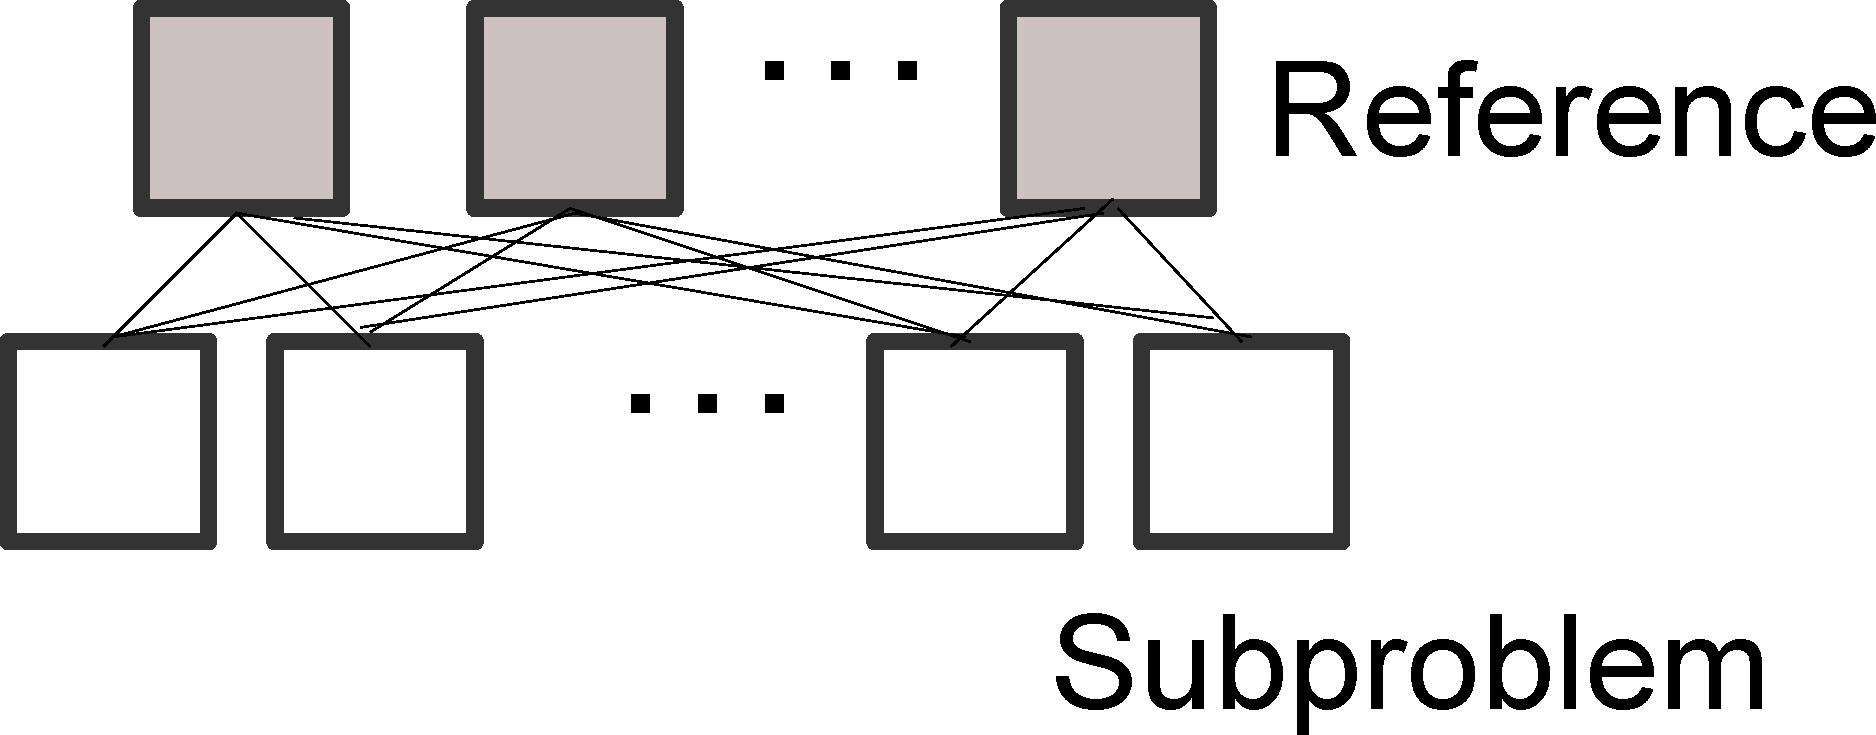
\includegraphics[width=0.7\linewidth]{fig/dependency}
\caption{The dependency of the trees in MORRF$^{*}$.}
\label{fig:dependency}
\end{figure}

Lemma \ref{lem:moo-d:rrt} tells us that the multi-objective path planning could be decomposed into a set of subproblems.
In MORRF$^{*}$, the responsibility of a subproblem tree is to find the optimal solution of its subproblem.
The next question needs to be answered is that whether the subproblem tree could find the optimal solution of its subproblem.

We notice that the \textsc{Extend} process in RRT$^{*}$ is not goal-oriented.
Let $ z^{*}(x) $ be the minimum cost from the start to the position of vertex $ x $.
We can generalize the conclusion of Theorem 22 in \cite{Karaman.Frazzoli:RSS10} to all the vertices in the RRT$^{*}$.
\begin{lem}
\label{lem:tree_vex:conv}
When Assumption \ref{asmp:additivity}, \ref{asmp:continuity} and \ref{asmp:spacing} hold,
the cost of the minimum cost path from the root to any vertex in RRT$^{*}$ converges to the optimal cost almost surely, i.e.,
$
P( \{ \lim_{ i \rightarrow \infty } c(x, i)  = z^{*}(x) \} ) = 1, x \in V $.
\begin{proof}
	%The construction of RRT* is not goal-oriented.
	%The ``rewire'' process potentially will update all the vertices and converge the value to the optimal one.
	%Similar with that of a goal vertex, the paths from the root to all other vertices will converge to corresponding optimal ones as well.
The asymptotic optimality of RRT$^{*}$ does not reply on how the sampling process is like (Theorem 22, \cite{Karaman.Frazzoli:RSS10}), though the convergence rate might be different.
Simply changing the goal to the position of any vertex still hold the asymptotic optimality.
Thus, we could generalize the asymptotic optimality from the goal to all the vertices.
\end{proof}
\end{lem}

The solve of a subproblem depends on a correct estimation of the reference vector $ \vec{z}^{*} $.
Thus, we need to have the solutions of all the reference trees converging to the optimal firstly.
The construction of a reference tree does not depend on any other tree.
Thus, the construction process is equivalent to the construction of a RRT*.
The asymptotic optimality of RRT* in Lemma \ref{lem:tree_vex:conv} is inherited here.
Thus the cost of the solution converges to the optimal of one single objective.
\begin{lem}
\label{lem:ref_tree:conv}
When Assumption \ref{asmp:additivity}, \ref{asmp:continuity} and \ref{asmp:spacing} hold,
the cost of the minimum cost path from the root to any vertex in $ k $-th reference tree converges to $ z^{*}_{k} $ almost surely, i.e., 
$ P( \{ \lim_{ i \rightarrow \infty }  c_{k} (x, i ) = z^{*}_{k} (x) \} ) = 1  $.
\end{lem}

Then we need to show that after all the reference trees converge to the structure that provides optimal cost, 
the subproblem tree can also converge to the structure that provides optimal fitness $ g^{*}_{m} ( x \mid \lambda_{m} , z^{*} ) $.
\begin{lem}
\label{lem:sub_tree:conv}
When Assumption \ref{asmp:additivity}, \ref{asmp:continuity} and \ref{asmp:spacing} hold,
with $ \vec{z}^{*} (x) $ for any $ x $ given,
the cost of the solution of $ m $-th subproblem tree converges to the optimal cost of the $ m $-th subproblem, i.e.,
$
P( \{ \lim_{ i \rightarrow \infty } c_{ \lambda_{m} }( i ) \} ) = z^{*}_{ \lambda_{m} }
$
\begin{proof}
When the reference vector $ \vec{z}^{*}(x) $ converges, the cost of the minimum cost path from the root to the vertex of position $ x $ in $ m $-th subproblem tree will gradually converge to the optimal by Lemma \ref{lem:tree_vex:conv}.
It means that the minimum fitness path from the root to any vertex in a subproblem tree will converge to an optimal minimum fitness path, in which the vertices in goal region are included.
It equals to that the cost of the solution of $ m $-th subproblem tree converges to the optimal cost of the $ m $-th subproblem.
%The construction of a subproblem tree depends on the convergence of all the reference trees.
%When all the reference trees have converged, the correct reference values $ c^{*} (x) $ of all the vertices could be obtained.
%The convergence process will be similar with that of a single RRT*.
%By Lemma \ref{lem:ref_tree:conv} and Lemma \ref{lem:sub_tree:conv}, we know that the utopia reference value $ c^{*} (x) $ could be correctly estimated after all the reference trees have reached optimality.
\end{proof}
\end{lem}

Now, we can prove that the solutions from MORRF$^{*}$ almost surely converges to a subset of the Pareto optimal set.

\begin{thm}
\label{thm:morrt:conv}
When Assumption \ref{asmp:additivity}, \ref{asmp:continuity} and \ref{asmp:spacing} hold,
the solutions from MORRF$^{*} $ converges to a subset of the Pareto optimal set almost surely, i.e.
$
P( \lim_{ i \rightarrow \infty }  \Sigma^{\mbox{MORRF}^{*}}_{i}  \subset \Sigma^{*} ) = 1.
$
\begin{proof}
As the solutions of MORRF$^{*}$ can be modeled in points in a high-dimension space by Lemma \ref{lem:moo-d:rrt}, the Tchebycheff method could be imported to decompose the multi-objective optimization problem into a set of subproblems.
By the fitness definition of the subproblem trees, if the subproblem tree could find a solution that minimize the fitness, the solution is in the Pareto optimal set of the multi-objective optimization problem.

Lemma \ref{lem:ref_tree:conv} guarantees that the reference vector $ \vec{z}^{*}(x) $ at any location $ x $ converges to the correct estimation after running enough iteration.
Thus, by Lemma \ref{lem:sub_tree:conv}, we have that the solution cost of the $ m $-th subproblem tree converges to $ z^{*}_{ \lambda_{m} } $.
It means that the solution converges to an optimal solution to $ m $-th subproblem as the iteration goes.
Therefore, the set of the solutions from all the subproblem trees converge to a subset of the Pareto optimal set, as the iteration goes~\cite{4358754}~\cite{miettinen1999nonlinear}.
\end{proof}
\end{thm}

\section{Simulation}
\label{sec:simulation}

\begin{comment}
2D (weighted sum + Tchebycheff method)
2D (With obstacles)
3D
compare NSGA-II
\end{comment}

Simulations have been taken to verify the performance of MORRF$^{*}$.
We 
We also implemented NSGA-II for multi-objective path planning, which is introduced in \cite{Ahmed2013}.
In order to be comparable, the path planning using NSGA-II is implemented in a continuous space.
Each solution is represented as a sequence of way points.
The cost is calculated like that in RRT*, whcih \textsc{Line}($ x_{1}, x_{2} $) is called to calculate the cost between two way points $ x_{1} $ and $ x_{2} $.


We tested firstly on path planning of two objectives.


We also tested with how MORRTF$^{*}$ works with obstacles.

 
More objectives are also tested here.

\section{Conclusion} 
\label{sec:conclusion}

This paper presented a MORRF$^{*}$ for the multi-objective path planning problems on continuous spaces.
The multi-objective optimization problem is decomposed into a few subproblems.
A forest of trees will explore the planning space to find the solution to corresponding subproblems.
The set of solutions from all the subproblem trees is a subset 

Boundary intersection approach -> better diversity

We can see that...
As a single query, the efficiency could be improved by sensing 

\section*{Acknowledgments}

%% Use plainnat to work nicely with natbib. 

\bibliographystyle{plainnat}
\bibliography{reference}

\end{document}